\def\lecturenumber{11}
\documentclass[11pt,a4paper]{article}
\usepackage[T1]{fontenc}
\usepackage[utf8]{inputenc}
\usepackage{lmodern}
\usepackage[margin=19mm,top=21mm,bottom=21mm,headheight=15pt]{geometry}
\usepackage{amsmath,amssymb,booktabs,array,graphicx,microtype}
\usepackage[dvipsnames]{xcolor}
\usepackage{enumitem,fancyhdr,listings,tcolorbox}
\usepackage[colorlinks=true,linkcolor=MidnightBlue,urlcolor=MidnightBlue]{hyperref}
\definecolor{courseblue}{HTML}{164B69}
\definecolor{pale}{HTML}{F0F5F7}
\pagestyle{fancy}
\fancyhf{}
\fancyhead[L]{\small\sffamily\color{courseblue}VALIDATED COMPUTING}
\fancyhead[R]{\small\sffamily Lecture \lecturenumber}
\fancyfoot[L]{\footnotesize Expanded lecture notes \textbullet\ October 2026}
\fancyfoot[R]{\footnotesize\thepage\ / 6}
\renewcommand{\headrulewidth}{0.4pt}
\setlength{\parindent}{0pt}
\setlength{\parskip}{5.5pt plus 1pt}
\setlength{\emergencystretch}{1.5em}
\setlist[itemize]{leftmargin=1.5em,itemsep=3pt,topsep=3pt}
\setlist[enumerate]{leftmargin=1.7em,itemsep=5pt,topsep=4pt}
\lstset{language=Python,basicstyle=\small\ttfamily,keywordstyle=\color{courseblue}\bfseries,
 commentstyle=\color{OliveGreen},stringstyle=\color{BrickRed},showstringspaces=false,
 columns=fullflexible,keepspaces=true,frame=single,rulecolor=\color{black!18},
 backgroundcolor=\color{black!2},aboveskip=6pt,belowskip=6pt,breaklines=true,
 xleftmargin=5pt,xrightmargin=5pt,framesep=5pt}
\newcommand{\R}{\mathbb R}
\newcommand{\fl}{\operatorname{fl}}
\newcommand{\abs}[1]{\left|#1\right|}
\newcommand{\heading}[2]{\section*{\color{courseblue}#1}\vspace{-4pt}{\small\sffamily\color{black!65}#2}\par\vspace{3pt}}
\newcommand{\opening}[2]{{\Large\sffamily\bfseries\color{courseblue}Lecture \lecturenumber\quad #1\par}\vspace{5pt}{\small #2}\par}
\newtcolorbox{question}[1]{colback=pale,colframe=courseblue!55,boxrule=0.4pt,
 arc=1mm,left=7pt,right=7pt,top=4pt,bottom=4pt,title={#1},fonttitle=\bfseries\small,
 coltitle=courseblue,colbacktitle=pale}
\newcommand{\reading}[1]{{\footnotesize\textbf{Reading and notebook.} #1\par}}
\hypersetup{pdfauthor={Validated Computing course},pdfsubject={Expanded introductory lecture notes with questions and exercises}}

\hypersetup{pdftitle={Lecture 11: Global minimum bounds and all minimizers}}
\begin{document}
\opening{Global minimum bounds and all minimizers}{Prerequisites: interval range enclosures and subdivision, Lectures 04--07.\newline
Goal: bound a global minimum and preserve every global minimizer during branch and bound.}
\heading{1. Two valleys expose two different questions}{0--13 minutes: the minimum value and the minimizing locations}
Consider the continuous objective
\[
                   f(x)=x^4-2x^2,\qquad x\in D=[-2,2].
\]
The identity $f(x)=(x^2-1)^2-1$ proves $f(x)\ge-1$, with equality exactly
at $x=-1$ and $x=1$. Thus the minimum value is $\mu=-1$ and the set of
global minimizers is $\{-1,1\}$. These are different mathematical objects:
one is a number, the other a set of input locations.

A local solver may find one valley and stop. Even an accurate candidate
does not prove there is no better value elsewhere, nor that another equally
good valley has been found. We will bound $\mu$ and retain a union of
intervals containing every minimizer. For this simple polynomial, the
identity supplies an independent reference against which to inspect the method.

\begin{center}
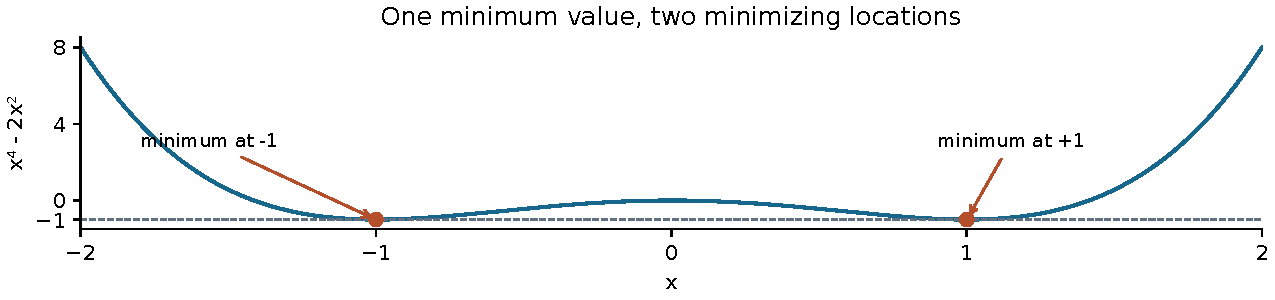
\includegraphics[width=0.92\linewidth]{figures/two_minima.pdf}
\end{center}

The existence premise matters. A continuous function on a nonempty compact
domain attains its minimum. Without it, the task might concern an unattained
infimum: $f(x)=x$ on $(0,1]$ has infimum zero but no minimizing point.
Our course algorithm assumes a closed, bounded interval and continuity there.

\textbf{Start with a deliberately wide expression.} A sharp square on
$[-2,2]$ gives $X^2=[0,4]$. Squaring that interval gives $X^4=[0,16]$.
Independent subtraction then yields
\[
                   F(X)=[0,16]-[0,8]=[-8,16].
\]
This is a valid range enclosure, but its lower endpoint $-8$ is far below
the minimum. Subdivision and better formulas can tighten it. Increasing
arithmetic precision cannot repair this exact-rational dependency loss.

\begin{question}{What does a successful local search prove?}
Suppose a solver returns $x\approx1$ and $f(x)\approx-1$. Which claims
about the global minimum and the other valley remain unproved? What changes
if the value at the proposed point is rigorously enclosed?
\end{question}

We will track a global lower bound, a feasible upper bound, and possible
minimizer locations separately. A narrow value interval need not imply
narrow location intervals, and a retained interval need not actually contain
a minimizer. Its meaning is that it has not safely been discarded.

\newpage
\heading{2. Lower bounds and feasible witnesses play different roles}{13--29 minutes: prove the pruning rule and preserve ties}
For every retained interval $X$, a valid image $F(X)=[L_X,H_X]$ gives
$L_X\le f(x)$ for all $x\in X$. These are lower bounds on entire regions.
To obtain an upper bound for the minimum, choose a feasible point $z\in D$
and rigorously enclose its value: $f(z)\in[l,u]$. Then
\[
                        \mu\le f(z)\le u=:U.
\]
The current best such upper bound is the \emph{incumbent}. A local solver
may propose $z$, but feasibility and its value enclosure must be checked.
The lower endpoint $l$ and midpoint of $[l,u]$ cannot in general replace $u$.

If the retained intervals cover every global minimizer, setting
$L=\min_X L_X$ gives $L\le\mu\le U$. At least one retained interval
contains a point where the minimum is attained; its lower bound cannot
exceed $\mu$. Other retained regions may make $L$ smaller than necessary,
which is why further refinement can help.

\textbf{Safe pruning.} If $L_X>U$, every value on $X$ is larger than
$U$, while a feasible witness has value at most $U$. No point in $X$ can
be a global minimizer, so we may discard $X$. Store both $L_X$ and the
incumbent used in the decision. Future improvements to the incumbent do
not invalidate this earlier exclusion.

The inequality must be strict when the promise is to retain \emph{all}
minimizers. A box with $L_X=U$ may contain another point attaining the same
minimum. For $(x^2-1)^2$, a known feasible value zero does not permit us
to discard every interval with lower bound zero: the two minimizing
locations $-1$ and $1$ would be lost.

\textbf{A concrete prune.} In our original objective, $z=1$ gives $U=-1$.
On $X=[0,1/4]$, the natural enclosure is $[-1/8,1/256]$. Its lower
endpoint satisfies $-1/8>-1$, so this entire central region can be removed.
The reason is a bound valid throughout the region, not the appearance of
the sampled graph near its midpoint.

\begin{question}{Why use the upper endpoint of a point value?}
A feasible point evaluation gives $[2,3]$. Which bound on $\mu$ follows
without additional information? Give a possible function value showing why
using $2$ as an incumbent could incorrectly discard a genuine minimizer.
\end{question}

\textbf{The invariant.} Initially the full domain contains all minimizers.
Replacing a retained interval by two covering children preserves them.
Strict pruning removes none of them. Induction therefore preserves every
global minimizer throughout the search. Budget exhaustion changes how
precise the result is, not the validity of the bounds already established.

\newpage
\heading{3. Build a small exact evaluator before the search}{29--43 minutes: rational endpoints and a hand trace}
The following code uses only \texttt{Fraction} arithmetic. The square
routine is the sharp one-variable operation from Lecture 04; the objective
then uses the expanded expression to leave visible work for subdivision.
All interval arguments below are ordered pairs of rational endpoints.
\begin{lstlisting}
from fractions import Fraction

def square_bounds(a, b):
    endpoint_squares = [a*a, b*b]
    if a <= 0 <= b:
        lower = Fraction(0)
    else:
        lower = min(endpoint_squares)
    return lower, max(endpoint_squares)

def objective_bounds(a, b):
    square_lower, square_upper = square_bounds(a, b)
    fourth_lower = square_lower * square_lower
    fourth_upper = square_upper * square_upper
    return (fourth_lower - 2*square_upper,
            fourth_upper - 2*square_lower)

def objective(x):
    return x*x*x*x - 2*x*x

assert objective_bounds(Fraction(-2), Fraction(2)) == (-8, 16)
assert objective(Fraction(1)) == -1
assert objective_bounds(Fraction(0), Fraction(1, 4)) == (
    Fraction(-1, 8), Fraction(1, 256))
\end{lstlisting}

Starting from the feasible point zero gives $U=0$. The first split of
$[-2,2]$ produces $[-2,0]$ and $[0,2]$. Their midpoints are $-1$ and $1$,
so evaluating them improves $U$ to $-1$. Both children still have natural
images $[-8,16]$: the global minimum enclosure is now $[-8,-1]$.
Sampling has improved the upper bound without yet improving the lower bound.

One more split of $[-2,0]$ gives $[-2,-1]$ with image $[-7,14]$ and
$[-1,0]$ with image $[-2,1]$. The other half $[0,2]$ still has lower
bound $-8$, so it deserves attention next. This motivates selecting a
region with the smallest lower bound: it is preventing a tighter global
certificate. The choice affects efficiency, not the minimizer invariant.

\begin{question}{Trace values and locations separately}
After the first split, which points supply the incumbent? Which intervals
remain possible minimizer locations? Why would keeping only the region
containing the first best witness fail the promise to retain both valleys?
\end{question}

The next loop is specialized to this polynomial on $[-2,2]$. Its initial
witness zero is feasible. A general implementation should also evaluate
domain endpoints, since a minimum can occur at a boundary; a derivative
equation alone does not cover that case.

\newpage
\heading{4. A visible branch-and-bound loop}{43--62 minutes: read the decisions and the stopping status}
This teaching implementation recomputes bounds each pass to keep its state
simple. Inputs are a positive rational tolerance and a nonnegative integer
split budget. Each split is exact and creates two nonempty covering children.
\begin{lstlisting}
def minimize_quartic(tolerance, max_splits):
    if tolerance <= 0 or max_splits < 0:
        raise ValueError("Invalid tolerance or split budget")
    pieces = [(Fraction(-2), Fraction(2))]
    pruned = []
    witness, upper = Fraction(0), Fraction(0)
    for splits in range(max_splits + 1):
        retained = []
        lower = None
        best_index = 0
        for a, b in pieces:
            local_lower, local_upper = objective_bounds(a, b)
            if local_lower > upper:
                pruned.append((a, b, local_lower, upper))
            else:
                retained.append((a, b))
                if lower is None or local_lower < lower:
                    lower = local_lower
                    best_index = len(retained) - 1
        pieces = retained
        if not pieces:
            raise ValueError("All candidates lost: inconsistent bounds")
        if upper - lower <= tolerance:
            status = "gap_met"
            break
        if splits == max_splits:
            status = "budget_exhausted"
            break
        a, b = pieces.pop(best_index)
        center = (a + b) / 2
        for left, right in [(a, center), (center, b)]:
            pieces.append((left, right))
            point = (left + right) / 2
            value = objective(point)
            if value < upper:
                witness, upper = point, value
    return pieces, pruned, witness, lower, upper, status
\end{lstlisting}

Point values are exact here, so the value itself is its safe upper endpoint.
With a machine evaluator, replace it by the upper endpoint of a point
enclosure. Every prune stores the evidence available at that moment; equality
retains the box. The loop checks the value gap before declaring the budget
exhausted, so reaching the target on the final allowed split counts as success.

\begin{question}{Locate the proof in the loop}
Identify strict pruning, both-child retention, feasible witness updates,
the global lower bound, and the actual gap test. Which line would become
unsafe if an approximate point value were substituted without an enclosure?
\end{question}

\newpage
\heading{5. Audit the value gap and the retained union}{62--77 minutes: run the calculation and read its limitations}
Continue the excerpts in the same session. The algebraically known minimum
provides a diagnostic; the search's guarantee comes from valid local bounds,
feasible witnesses, and minimizer preservation.
\begin{lstlisting}
result = minimize_quartic(Fraction(1, 100), 512)
pieces, pruned, witness, lower, upper, status = result
assert status == "gap_met"
assert lower <= -1 <= upper
assert upper - lower <= Fraction(1, 100)
assert -2 <= witness <= 2 and objective(witness) == upper
for minimizer in [Fraction(-1), Fraction(1)]:
    assert any(a <= minimizer <= b for a, b in pieces)

terminal = list(pieces)
for a, b, local_lower, old_upper in pruned:
    assert local_lower > old_upper
    terminal.append((a, b))
terminal.sort()
assert terminal[0][0] == -2 and terminal[-1][1] == 2
for index in range(len(terminal) - 1):
    assert terminal[index][1] == terminal[index+1][0]
print(status, str(lower), str(upper), len(pieces))
\end{lstlisting}

The terminal intervals, retained and pruned together, cover the full
original domain. The retained union alone need only contain every global
minimizer. A retained interval is a candidate, not a certificate that a
minimizer lies in it. Shared endpoints are harmless for coverage, but
counting candidate intervals would not count distinct minimizing points.

\textbf{What the gap means.} Since $L\le\mu\le U$, a gap $U-L\le\tau$
gives a value enclosure of width at most $\tau$. The feasible witness also
satisfies $0\le f(z)-\mu\le U-L\le\tau$. This says the witness is nearly
optimal in \emph{value}. It does not, without additional assumptions,
bound its distance to the minimizer set or shrink every candidate domain.

For the constant objective $f(x)=3$ on $[-10,10]$, the minimum value is
exactly known, but every point is a minimizer. An exact zero value gap is
therefore compatible with a retained interval of width 20. For $f(x)=x$
on $[0,1]$, the unique minimizer is the boundary point zero; evaluating only
interior stationary points would miss it entirely.

\begin{question}{Report a budget-limited run}
Run with tolerance $10^{-6}$ and a budget of two splits. State the valid
minimum interval and minimizer-cover claim, then state which requested
accuracy was not established. Why is the result still useful?
\end{question}

The notebook can intersect natural and mean-value enclosures before the
search. Tighter lower bounds may prune sooner; no theorem says every
additional bound pays for its cost. Compare the same objective, domain,
target, and arithmetic assumptions when assessing efficiency.

\newpage
\heading{6. Exercises and a global-optimization certificate}{77--90 minutes: choose two exercises; finish the rest independently}
\begin{enumerate}
\item \textbf{Prove the reference answer.} Use $(x^2-1)^2-1$ to prove
the minimum of $x^4-2x^2$ on $[-2,2]$ and identify every minimizing point.
Compare the natural range with the range obtained from this identity.
Why can the rewritten form make a global value certificate immediate once
a feasible witness at $1$ is available?

\item \textbf{Audit one strict prune.} With $U=-1$, compute the natural
image on $[0,1/4]$ and justify removing it. Then consider $(x^2-1)^2$
with incumbent zero. Explain why a region whose lower bound equals zero
must remain eligible if every minimizer is to be preserved.

\item \textbf{Find the missing feasible point.} Minimize $f(x)=x$ on
$[0,1]$. A routine seeks only roots of $f'$ and finds none. What has it
missed? If the routine starts with only the midpoint witness, which upper
bound does it obtain, and what does testing the left endpoint improve?

\item \textbf{Value accuracy versus location accuracy.} Let
$f(x)=\varepsilon x^2$ on $[-1,1]$, with $\varepsilon=10^{-8}$.
The point $z=1$ has value only $10^{-8}$ above the minimum, yet how far
is it from the minimizer? If a separate growth bound
$f(x)-\mu\ge c|x-x_*|^2$, $c>0$, is known, derive a location-error bound
from a witness value error at most $\tau$.

\item \textbf{Review an incomplete computation.} Run the standalone
loop with two allowed splits and tolerance $10^{-6}$. Determine $[L,U]$
and the retained intervals exactly. Explain why they still contain both
known minimizers, and why a zero-containing derivative interval would not
by itself establish a local or global minimum in any of them.
\end{enumerate}

\textbf{Selected checks.} Exercise 1: $\mu=-1$ at $\pm1$.
The natural range is $[-8,16]$; the rewritten expression gives $[-1,8]$,
which is the true range on the domain. Its lower bound and the witness
value prove $\mu=-1$. Exercise 2: $[-1/8,1/256]$ is strictly above the
incumbent in its lower endpoint. Exercise 3: the minimum is zero at the
left endpoint; the midpoint gives $U=1/2$, while that endpoint gives
$U=0$. Exercise 4: the distance is one; the extra growth assumption gives
$|z-x_*|\le\sqrt{\tau/c}$. Exercise 5: the retained domains are
$[0,2]$, $[-2,-1]$, and $[-1,0]$, with $[L,U]=[-8,-1]$ and status
\texttt{budget\_exhausted}. The small budget certifies a broad bound.

\begin{question}{Exit ticket: write the complete claim}
State the original domain and continuity premise, the enclosure of the
minimum value, the retained union containing all minimizers, the feasible
witness and its value bound, and the stopping status. Which part controls
value accuracy, and which part says where minimizers may be?
\end{question}

\reading{Companion: \texttt{notebooks/11\_global\_optimization.ipynb}
and Lab 11. Tucker (2011), \S5.2.1, pp.~87--89; monotonicity and convexity
tests in \S\S5.2.2--5.2.3 are extensions. SIAM Challenge Chapter 4 is an
optional later application. Next: reliable geometric decisions.}
\end{document}
